\chapter{Обзор задачи}

Задача о назначениях в самом общем виде формулируется следующим образом: есть некоторое количество \textit{работ} и некоторе количество \textit{исполнителей}. Любой исполнитель может быть назначен на выполнение любой (но только одной) работы, но с неодинаковыми затратами. Нужно распределить работы так, чтобы выполнить работы с минимальными затратами.

Строгая математическая формулировка звучит так.

Пусть даны множества $\mathrm{A}$, $\mathrm{T}$ и функционал стоимости $C:A \times T \rightarrow \mathbb{R}$. Необходимо найти биекцию $f: A \rightarrow T$, такую что 
$\sum_{a\in A}C(a,f(a))$ минимальна.

Рассмотрим матрицу $C \in Matr_{n \times m}$, тогда $c_ij$ -- стоимость назначения $i$ работника на $j$ работу, соотвественно целевая фунция переписывается ввиде 
$\sum_{a\in A}C_{a,f(a)}$.

Если число исполнителей и работ совпадает, $n=m$ , то задачу называют линейной. 

Эту задачу также можно переписать в виде задачи линейного программирования.

$$\sum_{i\in A}\sum_{j\in T}C(i,j)x_{ij}$$

и ограничениями 

\begin{align*}
& \sum_{j\in T}x_{ij}=1 \textnormal{ для } i\in A \\
& \sum_{i\in A}x_{ij}=1\textnormal{ для }j\in T \\
& x_{ij}\ge 0 \textnormal{ для } i,j\in A,T
\end{align*}

В терминах общей формулировки первое ограничение означает, что на каждый работник может быть назначен лишь на одну работу, а второе означает, что каждая работа может быть отдана лишь одному работнику. 

\section{Перестановки}

Введем понятие назначения. Мы можем
представлять назначение как некое биективное отображение $\phi$, которое ставит
элементы конечного множества $\mathrm{U}$ в соотвествие элементам конечного
множества $\mathrm{V}$. В тоже время назначение является перестановкой, которая записывается
в виде

\[
\left (
  \begin{tabular}{cccc}
  1 & 2 & \ldots & n\\
  $\varphi (1)$ & $\varphi (2)$ & \ldots & $\varphi (n)$
  \end{tabular}
\right )
\]



Каждой перестановке множества $\{1, 2, \ldots , n \}$ соответсвует единственная матрица
перестановок $\mathrm{X}_\varphi \in \mathrm{Matrix}_{n \times n}$, элементы котороый определяются как
\[
x_{ij} =
 \begin{cases}
   1 & \text{если } j = \varphi(i) \\
   0 & \text{иначе}
 \end{cases}
\]

Пример

\[
\left (
  \begin{tabular}{ccccc}
  1 & 2 & 3 & 4 & 5\\
  4 & 5 & 2 & 3 & 1
  \end{tabular}
\right )
\]


\[ \left(
\begin{matrix}
 0 & 0 & 0 & 1 & 0 \\
 0 & 0 & 0 & 0 & 1 \\
 0 & 1 & 0 & 0 & 0 \\
 0 & 0 & 1 & 0 & 0 \\
 1 & 0 & 0 & 0 & 0
\end{matrix} \right)
\]

\begin{figure}[h!]
  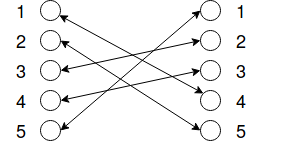
\includegraphics[width=0.3\textwidth]{Chapters/image/premutation.png}
  \caption{A boat.}
  \label{fig:flowchart}
\end{figure}


Обозначим множество $\mathrm{S}_n$ как множество всех возможных перестановок множества
 $\{1, 2, \ldots , n \}$. Мощность этого множества $n!$.

\subsection{Линейная задача о назначениях в терминах перестановок}
Пусть дана матрица $n \times n$ весовых коэфициентов $C = (c_{ij})$.
Требуется минимизировать линейную форму

\[
  \sum^n_{i = 1} c_{i \varphi (i)}
\]

то есть линейная задача о назначениях может быть поставлена в виде

\[
  \min_{\varphi \in S_n} \sum^n_{i = 1} c_{i \varphi (i)}
\].

При этом, если перестановки задаются матрицей перестановок $\mathrm{X} = (x_{ij})$,
линейная задача о назначениях может быть записана как задача линейной оптимизации
\begin{align}
  & \min \displaystyle \sum^n_{i = 1} \displaystyle \sum^n_{j = 1} c_{ij} x_{ij} \\
  \text{ограничения:} & \displaystyle \sum^n_{i = 1} x_{ij} = 1 &(j = 1, \ldots, n) \\
  &\displaystyle \sum^n_{j = 1} x_{ij} = 1 &(i = 1, \ldots, n) \\
  & x_{ij} \in \{ 0, 1 \}
  &(i,j = 1, \ldots, n)
\end{align}

Ограничения  $(2) \-- (4)$ задают допустимое множество

В дальнейшем будем называть $\mathrm{X}$ матрицей назначений.

\subsection{Трехиндексная задача о назначениях}

Аксиальная трехиндесная задача о назначениях может быть определена следующим образом. 
Пусть даны $n^3$ весовых коэфициентов $c_{ijk}, (i,j,k=1 \ldots n)$. 
Необходимо найти такие перестановки $\varphi$ и $\xi$, что 
\[
  \min_{\varphi, \xi \in S_n} \sum^n_{i = 1} c_{i \varphi (i) \xi(i)}
\]

где $S_n$ множество всех перестановок целых чисел от $1 \ldots n$.

Так же задача может быть переписана как задача целочисленного линейного программирования. 

\begin{eqnarray*}
  & \min \displaystyle \sum^n_{i = 1} \displaystyle \sum^n_{j = 1} \displaystyle \sum^n_{k = 1}
  c_{ijk} x_{ijk} \\
  \text{ограничения}
  &\displaystyle \sum^n_{i = 1} \displaystyle \sum^n_{k = 1} x_{ijk} = 1  &(j = 1, \ldots, n) \\
  &\displaystyle \sum^n_{j = 1} \displaystyle \sum^n_{k = 1} x_{ijk} = 1  &(i = 1, \ldots, n) \\
  &\displaystyle \sum^n_{i = 1} \displaystyle \sum^n_{j = 1} x_{ijk} = 1  &(k = 1, \ldots, n) \\
  & x_{ijk} \in \{ 0, 1 \} &(i,j,k = 1, \ldots, n)
\end{eqnarray*}


\begin{figure}[h!]
  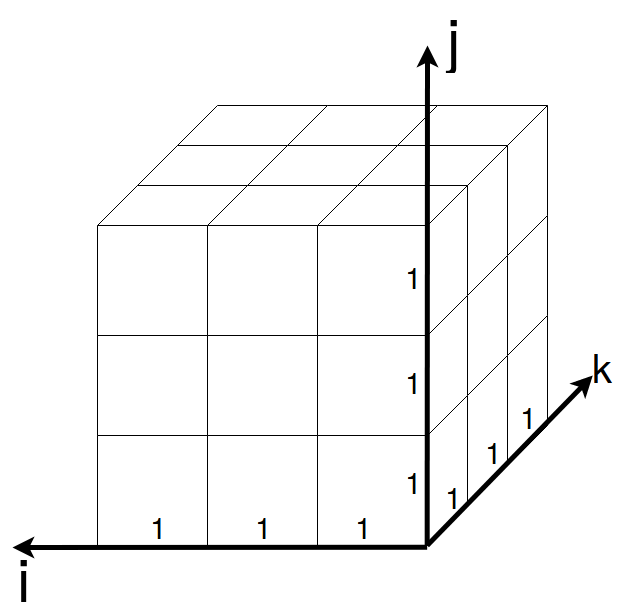
\includegraphics[height=0.3\textheight,keepaspectratio]{Chapters/image/example.png}
  \caption{A boat.}
  \label{fig:flowchart}
\end{figure}

3-АЗОН состоит в том, чтобы выбрать среди элементов трехмерной матрицы $C={c_{ijk}}$ такие $n^2$ элементов, что сумма в каждом выбраном сечении (при фиксированных $i,j,k$) минимальной. 

Известна следующая интерпритация этой задачи. Необходимо назначить работника $i$ на работу $j$ на машине $k$ так, 
чтобы стоимость назначения была минимальна.

Трехиндесная задача о назначениях также известна в планарной постановке. Содержательно она отличается от аксиальной тем, что что сумма всех выбранных элементов должна быть минимальна. 
